% !TeX root = main.tex
\chapter{A Single-Core with Gemmini RoCC Accelerator RISC-V Processor System}
\label{chap:SingleCoreGemminiRiscVSystem}

From the surveys and analyses in the preceding sections regarding processor cores and the two SoC development frameworks, it is evident that each of these research subjects possesses distinct advantages and limitations. However, for the research orientation and implementation of a processor system featuring a custom accelerator, the \texttt{Chipyard} framework and its library components are deemed most suitable for the objectives of this thesis. Not only does \texttt{Chipyard} effectively meet current requirements, but it also holds the potential for expansion to support more complex systems in the future.

This chapter will present a more detailed exposition of the component structure and the process of constructing an SoC system, while also delving into the architecture of the \texttt{Rocket} processor core. The thesis will utilize high-level design languages \texttt{Chisel}/\texttt{Scala} to implement a single-core processor system integrated with the \texttt{Gemmini} \texttt{RoCC} accelerator, focusing on leveraging the components within an SoC system, and building the hardware and software design based on the \texttt{Chipyard} framework.

\section{System Design Methodology with \texttt{Chisel}}
\label{sec:design_methodology_chisel}

As previously introduced, this thesis undertakes system design based on the components and tools within \texttt{Chipyard}. This framework and its library components are constructed from a diverse range of elements, all based on \texttt{Chisel}/\texttt{Scala}.

\subsection{\texttt{Chisel} and \texttt{Scala}}
\label{subsec:chisel_scala}

\begin{figure}[htbp]
    \centering
    \begin{subfigure}[b]{0.3\textwidth}
        \centering
        \includegraphics[width=\linewidth]{Images/Chisel_logo.pdf}
    \end{subfigure}%
    \hfill
    \begin{subfigure}[b]{0.18\textwidth}
        \centering
        
\includegraphics[width=\linewidth]{Images/Chisel_Scala_Logo.pdf}
    \end{subfigure}%
    \hfill
    \begin{subfigure}[b]{0.18\textwidth}
        \centering
        
\includegraphics[width=\linewidth]{Images/Chisel_FIRRTL.pdf}
    \end{subfigure}%
    \hfill
    \begin{subfigure}[b]{0.2\textwidth}
        \centering
        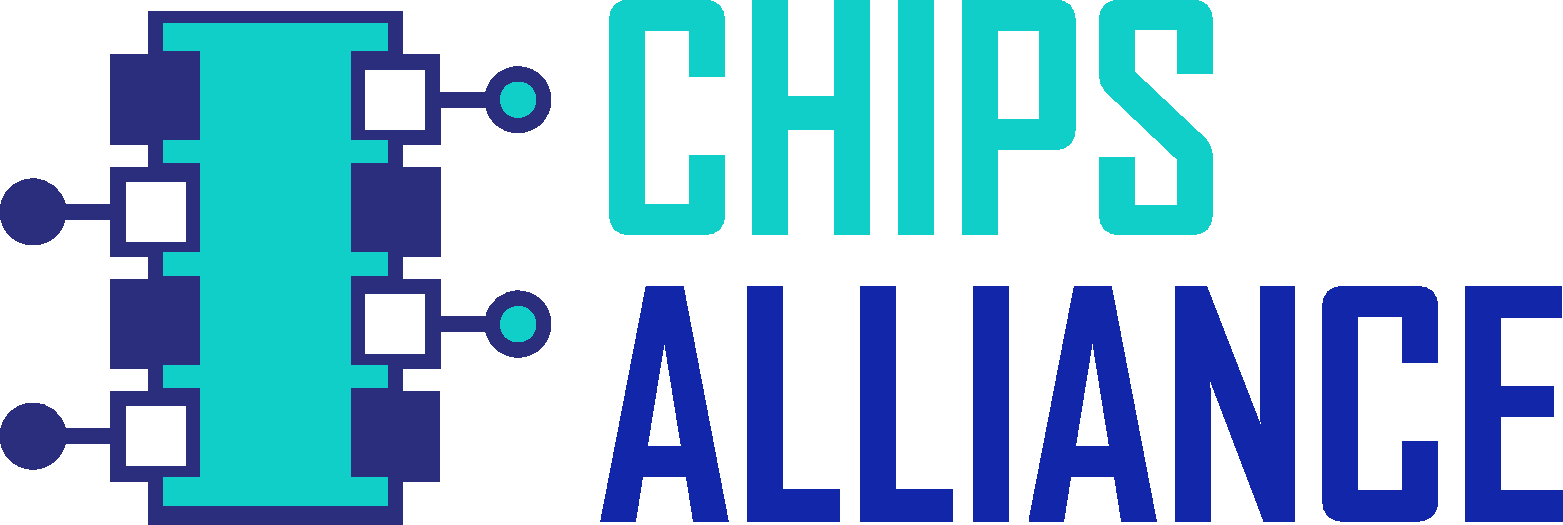
\includegraphics[width=\linewidth]{Images/Chisel_ChipsAlliance.pdf}
    \end{subfigure}
    \caption{\texttt{Chisel} as a library within \texttt{Scala}. Source: CHIPS Alliance.}
    \label{fig:chisel_ecosystem_logos}
\end{figure}

\texttt{Chisel} is a Hardware Construction Language (HCL) developed at UC Berkeley, initially intended to enable hardware design through highly parameterized and hierarchically specific code generators. \texttt{Chisel} is used to define these generators, which then produce designs in \texttt{Verilog}, suitable for industry-standard RTL design flows. \texttt{Chisel} is classified as a Domain-Specific Language (DSL); more precisely, it is implemented as a library package for \texttt{Scala}, a high-level, multi-paradigm programming language that integrates features of both Object-Oriented Programming (OOP) and functional programming on the \texttt{Java} Virtual Machine (JVM). Furthermore, \texttt{Scala}'s functional programming capabilities support higher-order functions and immutable data structures, facilitating more maintainable code, which is crucial for reproducibility and collaboration in scientific research.

\texttt{Chisel}'s design aims to address the lack of object-oriented programming and pre-processing structures in existing Hardware Description Languages (HDLs), supporting the construction of more flexible generators. By being based on \texttt{Scala}, \texttt{Chisel} gains the flexibility to describe hardware with high levels of abstraction and modularity. This helps hardware designers describe circuits in a way that is easy to maintain, modify, and extend, especially for large and complex designs such as microprocessors and specialized digital signal processing cores. \texttt{Scala}'s robust type system, diverse numerical representations and variables, immutability, and support for functional programming make it an ideal foundation for \texttt{Chisel}, aiding in error checking during hardware and circuit description and encouraging reusable design patterns.

In the context of hardware design based on \texttt{Chisel} and \texttt{Scala}, \texttt{sbt} (Simple Build Tool) plays a crucial role, optimizing the design management and development process. Built specifically for \texttt{Scala} and \texttt{Java} projects, \texttt{sbt} is the build tool used by the majority of \texttt{Scala} developers. Essentially, \texttt{sbt} acts as the compiler when working with \texttt{Chisel} and \texttt{Scala}. Using \texttt{sbt} simplifies the process of structuring projects for hardware design with \texttt{Chisel} in \texttt{Chipyard}, as well as enabling integration with many other open-source projects.

\subsection{\texttt{Verilator} Simulation Tool}
\label{subsec:verilator}

In the hardware design process, evaluating the functionality of the design is critically important. With \texttt{Chipyard}, system designs, from simple to complex structures, can be effectively realized and tested thanks to integrated tools and RTL simulators like \texttt{Verilator}, which are readily available within the project framework.

\texttt{Verilator} is an open-source program, prominent in the field of RTL simulation due to its unique method of converting ("Verilating") \texttt{Verilog} or \texttt{SystemVerilog} into \texttt{C++} or \texttt{SystemC}, creating a highly optimized executable program. Unlike traditional simulators, \texttt{Verilator} does not directly interpret \texttt{Verilog} during simulation. Instead, it generates \texttt{C++} or \texttt{SystemC} program files by parsing the hardware code, performing syntax checking, linting, and optionally inserting debug points and coverage analysis to enhance the correctness and accuracy of evaluation and verification. This "Verilated" output file can be configured to run in single-threaded or multi-threaded mode on a development server, offering an advantage for simulating complex or computationally demanding designs. After the "Verilated" code is generated, it is compiled by a standard \texttt{C++} compiler such as \texttt{GCC}, \texttt{Clang}, or \texttt{MSVC++}, and is typically combined with a user-provided wrapper file to manage the initialization of the Verilated model.

\texttt{Verilator} offers high simulation performance, especially for designs requiring substantial resources, due to its high speed and cycle accuracy. \texttt{Verilator}'s compilation approach makes it up to 100 times faster than interpretive simulators like Icarus \texttt{Verilog} (which is also open-source), and with multi-threading, performance can increase by an additional 2-10 times, achieving a total improvement of up to 1000 times. This makes \texttt{Verilator} suitable for RISC-V multi-core processor designs ranging from simple to complex, and competitive even with commercial simulators such as Synopsys VCS, Cadence Incisive, or Mentor ModelSim.

\section{The \texttt{Rocket} Processor Core}
\label{sec:rocket_core}

As introduced in the previous chapter, \texttt{Rocket} is a 5-stage, in-order processor core compliant with the RISC-V instruction set architecture, with RV32G and RV64G variants. Currently, the development of the \texttt{Rocket} core is maintained by the CHIPS Alliance. \texttt{Rocket} is written in the \texttt{Chisel} hardware design language, based on the \texttt{Scala} programming language, and is a key component of the \texttt{Rocket Chip} SoC Generator toolchain.

When implemented, each \texttt{Rocket} core is combined with L1 data and instruction caches. This memory operates locally for each core and, in a multi-core system, is responsible for storing temporary variables generated during the execution of the pipeline, helping to reduce congestion when multiple cores attempt to store data. Together with the Page Table Walker (\texttt{PTW}), a Tile within the SoC is formed. This \texttt{Rocket} Tile (Figure \ref{fig:rocket_tile_structure}) is considered a fundamental unit in the \texttt{Rocket Chip} SoC system and can be replicated to create multi-core processor systems, meeting the demands for performance and flexibility in modern SoC design.

\begin{figure}[h!]
    \centering
    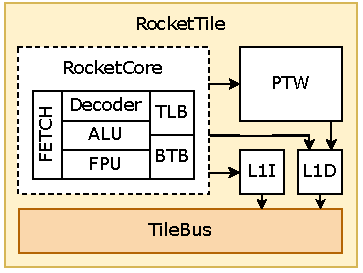
\includegraphics[width=0.7\textwidth]{Images/RocketTile_Basic.pdf}
    \caption{Structure of a \texttt{Rocket} Tile.}
    \label{fig:rocket_tile_structure}
\end{figure}

Due to the object-oriented nature of \texttt{Chisel}, the language used for its design, \texttt{Rocket} itself is written from object classes that can be defined and reconfigured according to implementation needs, such as \texttt{WithNBigCore()}, \texttt{WithNMedCore()}, \texttt{WithNSmallCore()}, and \texttt{WithNTinyCore()}. Additionally, instead of implementing the \texttt{Rocket} core, the \texttt{BOOM} core can also be integrated in its place, and many other peripherals can be integrated into a Tile unit.


\section{\texttt{Rocket Chip} SoC Structure}
\label{sec:rocketchip_soc_structure}

This system generator includes multiple components, not just the processor core but also the on-chip system bus (SoC bus), specifically \texttt{TileLink}. \texttt{TileLink} comprises a peripheral bus, control bus, and memory bus, along with arbiters and system controllers. Additionally, the system integrates peripheral components such as DRAM, GPIO, UART, and, critically for this thesis, supports tightly-coupled accelerators like \texttt{Gemmini} via the \texttt{RoCC} interface. Figure \ref{fig:single_core_gemmini_system} below depicts the generalized structure of the single-core RISC-V processor system with a \texttt{Gemmini} \texttt{RoCC} accelerator, which forms the basis for the development in this thesis.

\begin{figure}[h!]
    \centering
    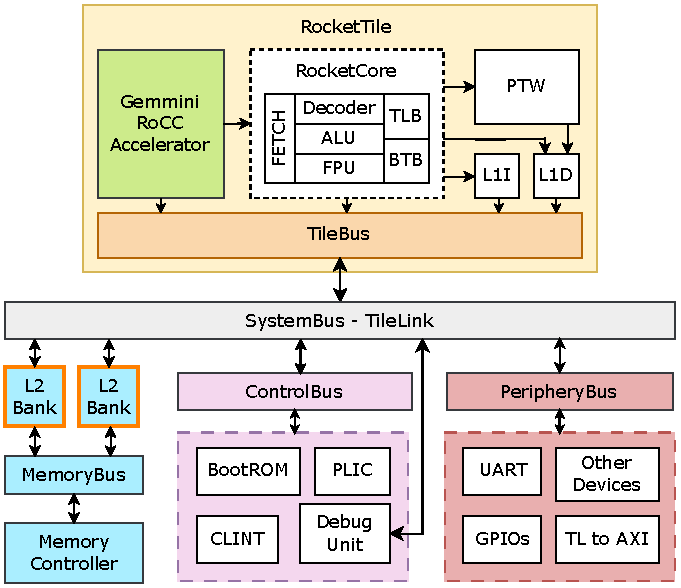
\includegraphics[width=0.9\textwidth]{Images/RocketChip_Gemmini_Diagram.pdf}
    \caption{Proposed structure of a single-core RISC-V processor system with a \texttt{Gemmini} \texttt{RoCC} accelerator.}
    \label{fig:single_core_gemmini_system}
\end{figure}

\subsection{Bus and Interconnect}
\label{subsec:bus_interconnect}

In the design of Systems-on-Chip (SoCs), bus architecture plays a backbone role, connecting and coordinating the operation of all components within the system. Particularly for modern multi-core processor systems, development trends focus on using crossbar-type bus architectures instead of Time Shared Buses. A crossbar, specifically a fully-connected crossbar structure, is considered a form of hardware switching fabric, allowing any input port to connect directly to any output port simultaneously. The outstanding advantage of this architecture lies in its ability to provide high bandwidth and low latency, effectively meeting performance requirements in applications such as networking equipment, multi-core processors, and high-performance storage systems. The optimization in data transmission offered by this architecture is a key factor in improving the overall performance of modern SoC systems.

For \texttt{Rocket Chip}, the \texttt{TileLink} \cite{sifive2018tilelink} system communication bus was developed concurrently with the project and the RISC-V instruction set, and is widely used in open-source system research at present.

\begin{figure}[h!]
    \centering
    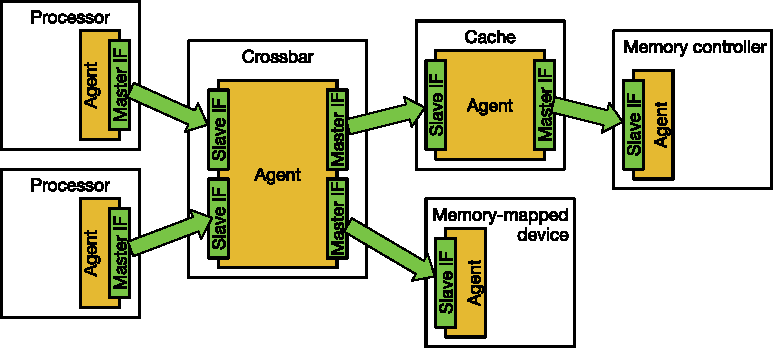
\includegraphics[width=0.8\textwidth]{TileLink_Topology.pdf}
    \caption{Connection model in \texttt{TileLink} and its interfaces. Source: \cite{sifive2018tilelink}}
    \label{fig:tilelink_connection_model}
\end{figure}

\texttt{TileLink} is a highly parameterizable, open-source, shared memory interconnect protocol based on the aforementioned crossbar structure, designed to connect diverse modules for SoCs. \texttt{TileLink} is implemented via a hierarchical, point-to-point network that can be easily scaled. This protocol provides memory-mapped access for multiple controllers, ensuring memory coherency while supporting efficient communication between processors, DMAs, and peripheral devices.

A \texttt{TileLink} bus system can support a combination of multiple communicating agents, each capable of supporting different configured subsets of the protocol. The \texttt{TileLink} specification includes three levels of operational configuration for agents, presented in Table \ref{tab:tilelink_configs}.

\begin{table}[h!]
\centering
\caption{\texttt{TileLink} operational configurations. Source: \cite{sifive2018tilelink}}
\label{tab:tilelink_configs}
\begin{tabular}{|l|c|c|c|}
\hline
 & \textbf{TL-UL} & \textbf{TL-UH} & \textbf{TL-C} \\
\hline
\textbf{Read/Write operations} & y & y & y \\
\textbf{Multibeat messages} & . & y & y \\
\textbf{Atomic operations} & . & y & y \\
\textbf{Hint operations} & . & y & y \\
\textbf{Cache block transfers} & . & . & y \\
\textbf{Channels B+C+E} & . & . & y \\
\hline
\end{tabular}
\end{table}

\texttt{TileLink} clearly distinguishes between cached and uncached communications. The simplest level is \texttt{TileLink} Uncached Lightweight (\texttt{TL-UL}), which only supports basic read and write operations to memory, for individual words. The next, more complex level is \texttt{TileLink} Uncached Heavyweight (\texttt{TL-UH}), which adds features such as "hints," "atomic" operations, and burst accesses but does not support coherent caching. Here, "hints" refers to a feature where a request command seeks data information external to the executing command from masters, and "atomic" refers to operations that lock access rights in a system with multiple masters, which could be microprocessors. Finally, \texttt{TileLink} Cached (\texttt{TL-C}) is the full protocol, supporting the use of coherent caches within the system.

For integrating peripheral hardware, all three bus configuration levels can be used. The communication connection diagram, at its most complete level, between a custom peripheral hardware and an agent is shown in Figure \ref{fig:tilelink_channels}.

\begin{figure}[h!]
    \centering
    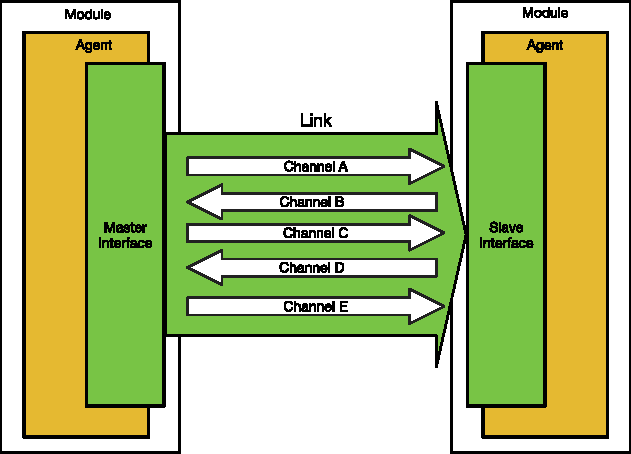
\includegraphics[width=0.8\textwidth]{TileLink_FiveChannel.pdf}
    \caption{Channels in a \texttt{TileLink} connection between two agents. Source: \cite{sifive2018tilelink}}
    \label{fig:tilelink_channels}
\end{figure}

In this \texttt{TileLink} protocol, the defined communication channels include \texttt{A}, \texttt{B}, \texttt{C}, \texttt{D}, and \texttt{E}, each undertaking specific roles in the interaction process between a master (M) and a slave (S), and all have a defined direction of transmission as depicted in the figure above.
\begin{itemize}
    \item \textbf{Channel A:} This is the initiation channel, where M sends requests to S, establishing the initial step of the communication process.
    \item \textbf{Channel B:} This channel is used when M requests a cache block from S, ensuring necessary data is queried.
    \item \textbf{Channel C:} Used for S to respond to M's request for a cache block, playing a crucial role in providing necessary data to M.
    \item \textbf{Channel D:} This is the general response channel, where S sends the final response to M after processing requests.
    \item \textbf{Channel E:} This channel ensures transaction completion by performing the final handshake for cache block transfer between the two parties.
\end{itemize}

The priority order for these channels is as follows: \texttt{A} < \texttt{B} < \texttt{C} < \texttt{D} < \texttt{E}, where channel \texttt{A} has the lowest priority and \texttt{E} has the highest. Prioritization in the \texttt{TileLink} bus system ensures that messages transmitted through the system do not fall into a hold-and-wait loop. In other words, the message flow through all channels between agents is maintained as a directed acyclic graph, enabling the \texttt{TileLink} protocol to operate without encountering deadlocks, ensuring continuous and uninterrupted data flow within the system.

% The choice of TileLink bus configuration depends on the component desired to be connected to the system; in this thesis, these are cryptographic algorithm accelerator cores designed separately using Verilog HDL. For this purpose, the TileLink configuration used for integration is TL-UL, which only includes channels A and D between M and S, as shown in Figure \ref{fig:tilelink_tl_ul_structure}.

The choice of \texttt{TileLink} bus configuration is relevant for connecting various memory-mapped peripherals within the system. For general-purpose MMIO peripherals, which might include cryptographic algorithm accelerators designed in \texttt{Verilog} HDL (if they were to be integrated as MMIO devices), the \texttt{TL-UL} configuration, comprising only channels \texttt{A} and \texttt{D} between M and S (as shown in Figure \ref{fig:tilelink_tl_ul_structure}), is often sufficient. However, for the primary accelerator in this thesis, the \texttt{Gemmini} core, integration is achieved through the \texttt{RoCC} interface, which provides a more tightly-coupled path to the processor core, rather than as a \texttt{TileLink}-attached MMIO peripheral. Details on the \texttt{RoCC} interface are discussed further in Section \ref{subsec:peripheral_components}. For other standard MMIO peripherals, a wrapper from the \texttt{Rocket Chip} library, using \texttt{Chisel}/\texttt{Scala}, can be inherited and customized to connect their signals to the appropriate system bus, typically the peripheral bus.


\begin{figure}[h!]
    \centering
    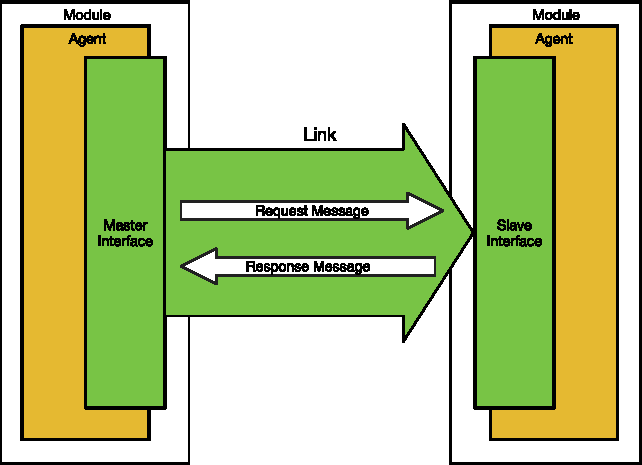
\includegraphics[width=0.7\textwidth]{TileLink_Overview.pdf} % Replace placeholder.png with your actual image file
    \caption{\texttt{TileLink} \texttt{TL-UL} connection structure. Source: \cite{sifive2018tilelink}}
    \label{fig:tilelink_tl_ul_structure}
\end{figure}

At the system configuration level, a wrapper from the \texttt{Rocket Chip} library, using \texttt{Chisel}/\texttt{Scala}, can be inherited and customized to convert the signals of the accelerator core to the system bus, in this case, the peripheral bus. Details for this interface will be further elaborated in subsequent sections of this thesis.

\subsection{Memory and Cache}
\label{subsec:memory_cache}

Each Tile in the system is integrated with a processor core and an L1 cache that is flexibly configurable. By default design with \texttt{Chisel}, the L1 cache has a size of 16 KiB, organized multi-dimensionally with sets and ways. The L1 cache uses a set-associative cache structure, dividing the memory region into sets, each set containing a fixed number of data blocks (ways). When a memory address access request occurs, the index derived from the address maps it to a specific set. The cache controller then searches for the data block within the ways of that set. This design supports both instruction and data storage, optimizing access performance and increasing the hit rate compared to caches with lower associativity.

In addition to the L1 cache, the system also integrates a shared L2 cache, connected to all cores via the \texttt{TileLink} bus system. The L2 cache acts as an intermediate storage repository, allowing processor cores and other components in the system to perform read/write data requests. This is a coordination mechanism that helps reduce pressure on the main memory and improves overall processing performance. The L2 cache controller also ensures fairness in resource allocation, using a queuing system to manage access requests.

At a higher level, the system also supports the integration of external memory, such as DRAM or SRAM, through open-source controllers or specialized IPs from FPGA implementation toolkits. Additionally, an interface with \texttt{DRAMSim} is supported for integration when performing full-system simulation. This provides flexibility and scalability, meeting various requirements in practical applications.

\subsection{Core-Complex}
\label{subsec:core_complex}

As previously mentioned, the \texttt{Chipyard} framework and library consist of many component definition classes that can form a \texttt{Rocket Chip} system. This allows for the formation of a complex system with diverse processor cores and peripherals, specifically heterogeneous architecture systems comprising multiple different processors like \texttt{Rocket} and \texttt{BOOM} coexisting on the system.

In these multi-core processor structures, each individual core will be uniquely identified with a different hart ID, ordered according to the system configuration. An example can be referenced below with a configuration comprising one \texttt{Rocket} core and one \texttt{BOOM} core. The corresponding block diagram configuration when generating the system will be as shown in Figure \ref{fig:heterogeneous_cores_system} below.

% Same, which one sounds better?
% As previously mentioned, the Chipyard framework and library consist of many component definition classes that can form a Rocket Chip system. This allows for the formation of a complex system with diverse processor cores and peripherals. A key capability is the creation of systems with heterogeneous architectures, potentially comprising multiple different processor cores like Rocket and BOOM coexisting on the same system, as illustrated in Figure \ref{fig:heterogeneous_cores_system}.

% In such multi-core processor structures, each individual processor core would be uniquely identified with a different hart ID, ordered according to the system configuration. For instance, a configuration might include one Rocket core alongside a BOOM core.

\begin{figure}[h!]
    \centering
    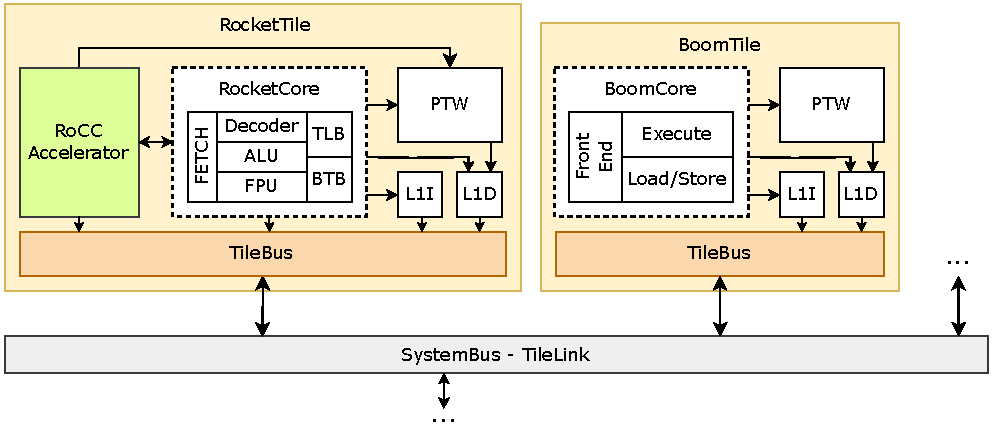
\includegraphics[width=0.8\textwidth]{RocketBOOM_CoreComplex.pdf} % Replace placeholder.png with your actual image file
    \caption{Implementation structure of a heterogeneous multi-core processor system.}
    \label{fig:heterogeneous_cores_system}
\end{figure}

A heterogeneous SoC system is an implementation approach also considered in this thesis to combine different processor cores to optimize performance and energy efficiency. At the application scale, lightweight cores can handle simple tasks with low power consumption, while high-performance cores support hyper-threading and out-of-order execution to process complex tasks. This design ensures flexibility, resource optimization, and superior performance for diverse applications.

\subsection{Peripheral Components}
\label{subsec:peripheral_components}

In the base system configuration class of \texttt{Rocket Chip}, many peripheral components are initialized and integrated by default to support both simulation and deployment on FPGA hardware for the SoC system. This configuration includes basic I/O devices such as PWM, interrupt controllers, JTAG, ROM, external memory, and standard peripheral interfaces, ensuring that basic communication, storage, and control requirements are met. In particular, common peripheral devices like UART, SPI Flash, and GPIO are implemented to support serial communication, storage management, and flexible control within the system.

\begin{figure}[h!]
    \centering
    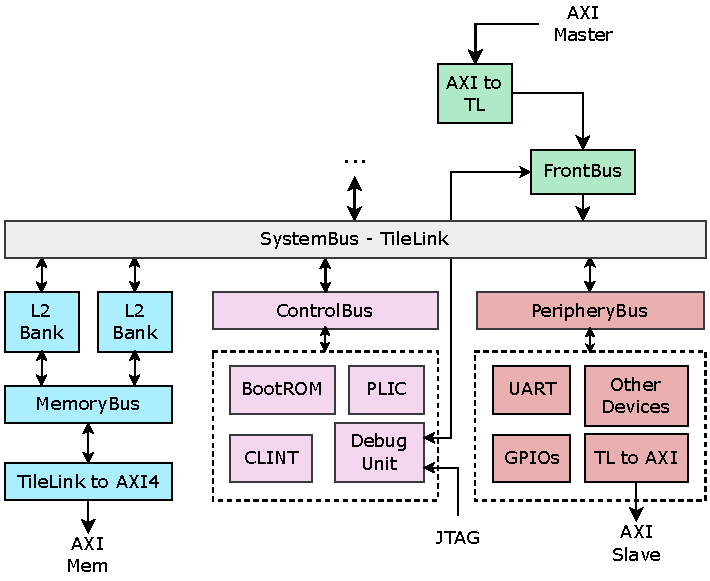
\includegraphics[width=0.8\textwidth]{RocketChip_Peripherals.pdf}
    \caption{Peripherals in the Rocket Chip base system.}
    \label{fig:rocketchip_base_peripherals}
\end{figure}

%  \begin{figure}[h!]
% \centering
% \includegraphics[width=0.8\textwidth]{placeholder.png} % Still using placeholder for this general example
% \caption{Implementation structure of a heterogeneous multi-core processor system (e.g., Rocket and BOOM). This illustrates a general capability of Chipyard.}
% \label{fig:heterogeneous_cores_system} % Kept the original label, adjust if needed
% \end{figure}

% A heterogeneous SoC with multiple distinct processor cores is an advanced implementation option that can be used to optimize performance and energy efficiency. At an application scale, lightweight cores could handle simple tasks with low power consumption, while high-performance cores could support features like hyper-threading and out-of-order execution for complex tasks. While the system developed in this thesis focuses on a single Rocket core augmented by the Gemmini RoCC accelerator, understanding Chipyard's capacity for heterogeneous multi-processor designs highlights its flexibility and potential for future, more complex applications. The design principles of modularity and clear interfacing within Chipyard facilitate such varied configurations.

All these components are developed based on the open-source \texttt{Rocket Chip} library, with hardware designs like \texttt{Rocket} and \texttt{BOOM} realized on the \texttt{Chisel} platform. When external memory is needed in design and simulation, the \texttt{AXI4} (Advanced eXtensible Interface 4) interface can be integrated as an intermediate layer, allowing effective connection with DRAM or SPI Flash models. Concurrently, serial protocols like JTAG are integrated to ensure accurate debugging capabilities and efficient serial communication, configured to connect with the \texttt{TileLink} bus. The \texttt{Rocket Chip} system also supports flexible configuration through special control ports, including custom boot pins and chip identification ports. Furthermore, the \texttt{Rocket Chip} system provides the capability to directly map bus interfaces such as \texttt{AXI4} Memory and MMIO (Memory-Mapped IO), allowing for expanded compatibility and optimized performance in complex SoC applications.

To expand the capability of integrating components and peripheral cores to form highly parameterized custom systems suitable for specific applications, the \texttt{Rocket Chip} architecture provides two flexible methods for peripheral integration. Specifically, the system can integrate a peripheral core as a \texttt{RoCC} (\texttt{Rocket} Custom Co-processor), located within each tile, or integrate at the system communication level via the MMIO mechanism. These methods facilitate in-depth customization, meeting various requirements for each specific application.

\begin{figure}[h!]
    \centering
    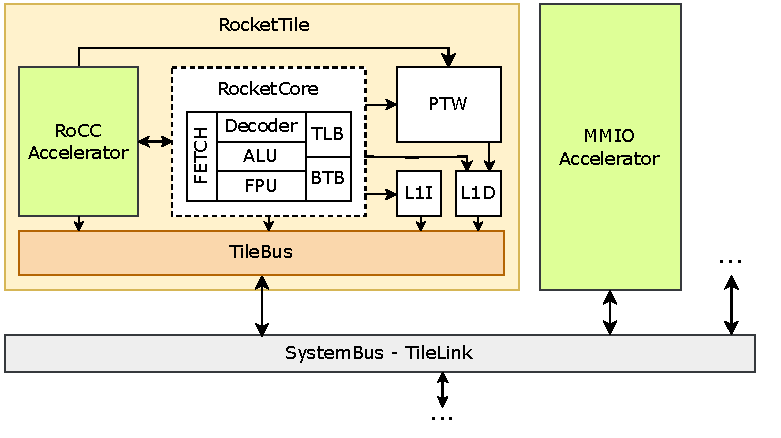
\includegraphics[width=0.8\textwidth]{RocketChip_WithMMIO.pdf} % Replace placeholder.png with your actual image file
    \caption{\texttt{RoCC} co-processor core and MMIO peripheral core in \texttt{Rocket Chip}.}
    \label{fig:rocc_mmio_rocketchip}
\end{figure}

MMIO Peripherals are custom peripherals attached directly to the \texttt{TileLink} bus, while Tightly-Coupled \texttt{RoCC} Accelerators are custom peripherals attached directly to the arbiter and processor within each Tile, in parallel with the processor core. With the \texttt{TileLink}-Attached MMIO method, the processor communicates with MMIO devices through registers mapped into memory at addresses on the system. Through these registers, control mechanisms or data transfer can be customized to suit the application of the peripheral core. Conversely, in the \texttt{RoCC} Accelerator method, communication is performed via a custom protocol and non-standard ISA instructions, which are configured and defined separately within the encoding space of the RISC-V ISA. For \texttt{Rocket} and \texttt{BOOM}, each core can control up to four accelerators through custom opcodes, sharing resources with the microprocessor. Instructions executed with \texttt{RoCC} cores have the format \texttt{customX rd, rs1, rs2, funct}. Here, \texttt{X} is a number from 0-3, determining the opcode that controls the routing of the instruction to a specific accelerator. The fields \texttt{rd}, \texttt{rs1}, \texttt{rs2} are the register numbers for the destination register and two source registers, and the \texttt{funct} field is a 7-bit integer that the accelerator can use to differentiate various instructions.

Peripherals connected as \texttt{RoCCs} have a distinct advantage due to their high customizability and direct connection and control via custom ISA instructions. This allows for specialized performance optimization, particularly useful for cores requiring large, complex computational workloads or applications needing extremely fast response times. Communication via a custom protocol and leveraging the RISC-V ISA helps \texttt{RoCC} utilize CPU resources efficiently, while also offering flexibility in designing specialized accelerator processors. The \texttt{Gemmini} accelerator, central to this thesis, is a prime example of a \texttt{RoCC}-based component, designed for high-throughput matrix multiplication and tightly integrated with the \texttt{Rocket} core.

While \texttt{RoCC} implementation can require a custom software toolchain for its specialized instructions, the performance benefits for demanding applications like those targeted by \texttt{Gemmini} often justify this investment. For this thesis, the integration of the \texttt{Gemmini} accelerator via the \texttt{RoCC} interface is deemed the most appropriate approach to achieve the desired performance for deep learning workloads.

Conversely, the MMIO \texttt{TileLink}-Attached method is widely used for integrating general-purpose memory-mapped peripheral devices. In this model, peripheral devices provide a set of registers (e.g., \texttt{Chisel} Registers) to communicate with microprocessors or other masters on the system bus. This method is suitable for peripherals where the tight coupling and custom instruction set of \texttt{RoCC} are not necessary.

To minimize design complexity for MMIO peripherals, the \texttt{Rocket Chip} architecture provides the \texttt{regmap} interface, which allows for the automatic generation of much of the necessary linking logic. Designers can use \texttt{TLRegisterRouter} or create a \texttt{LazyModule} and initialize \texttt{TLRegisterNode} to integrate such devices. Since \texttt{TileLink} is the official protocol used in SoCs based on \texttt{Rocket Chip} and \texttt{Chipyard}, designing MMIO peripheral devices (other than the primary \texttt{RoCC} accelerator) would typically focus on integration with this protocol.

% Original version
% However, this method also comes with some notable drawbacks. Firstly, implementing RoCC requires a custom software toolchain to synthesize special execution instructions, leading to longer development times and potentially increasing system complexity. Secondly, leveraging RoCC is only truly necessary for applications demanding extremely high performance; for use cases not requiring special optimization, this method may not provide value commensurate with the investment of effort. Dependence on non-standard instructions can reduce compatibility and scalability in diverse system designs. The development and integration of peripherals using the MMIO TileLink approach is deemed more suitable for the purposes of this thesis.

% The MMIO TileLink-Attached method is widely used in designing memory-mapped peripheral devices. In this model, peripheral devices provide a set of registers, specifically Chisel Registers, to communicate with microprocessors or other masters on the system bus. By writing data to these registers, microprocessors can adjust settings or send commands to the peripheral device or accelerator core. Conversely, by reading from these registers, the microprocessor can query the status or receive results and data from the peripheral device or accelerator core.

% To minimize design complexity, the Rocket Chip architecture provides the "regmap" interface, which allows for the automatic generation of much of the necessary linking logic. Instead of manually writing management nodes and register-exposing logic, designers can easily use TLRegisterRouter or create a LazyModule and initialize TLRegisterNode to integrate the device into the system. The simplest way to create an MMIO peripheral device is to use a configuration class like TLRegisterRouter, or AXI4RegisterRouter if choosing to use the AXI4 bus. This abstracts the details of the interconnect protocol with the peripheral bus (PBUS) and provides a convenient interface for defining memory-mapped registers. Since TileLink is the official protocol used in SoCs based on Rocket Chip and Chipyard, designing MMIO peripheral devices typically focuses on integration with this protocol, ensuring consistency and efficiency throughout the system.